\documentclass[12pt,a4paper]{article}

\usepackage[utf8]{inputenc}
\usepackage[T1]{fontenc}
\usepackage[brazil]{babel}
\usepackage{amsmath,amssymb}
\usepackage{graphicx}
\usepackage{booktabs}
\usepackage{siunitx}
\usepackage{geometry}
\usepackage{hyperref}
\usepackage{caption}
\captionsetup{font=small,labelfont=bf}

\geometry{margin=2.4cm}

\title{\textbf{Ajuste de Franjas de Ramsey em Chafariz Atômico:\\ Simulação Otimizada com Pulso Não-Instantâneo\\ e Resposta Instrumental Linear}}
\author{Relatório técnico — projeto \texttt{fountain\_sim}}
\date{\today}

\begin{document}

\maketitle

\begin{abstract}
Este relatório documenta o desenvolvimento de uma metodologia completa para ajustar as
franjas de Ramsey simuladas aos dados experimentais de um chafariz atômico de césio.
Foram implementadas (i) uma simulação otimizada do perfil não-instantâneo de ativação do
campo de micro-ondas, usando quadraturas de Gauss--Hermite e Gauss--Legendre e avaliação
direta nas dessintonias de interesse; (ii) uma modelagem da \emph{resposta instrumental}
linear do detector, $y = A\,P_2 + C$, com os parâmetros $A$ (contraste) e $C$ (fundo)
perfilados analiticamente; e (iii) um procedimento de seleção de modelo entre sete perfis
de ativação distintos. O resultado principal é a elevação da qualidade do ajuste de
$R^2 \approx 0{,}80$ (com normalização min--max) para $R^2 \approx 0{,}98$ (com resposta
instrumental), com RMSE da ordem de $0{,}005$ no sinal bruto. O relatório detalha as
funções implementadas, as métricas de eficácia e os gráficos que comprovam a viabilidade
do método.
\end{abstract}

\tableofcontents

\section{Introdução}
Um chafariz atômico lança verticalmente uma nuvem de átomos de césio-133, que atravessa
duas vezes uma cavidade de micro-ondas (na subida e na descida), realizando uma
interferometria de Ramsey. O padrão de interferência resultante --- as \emph{franjas de
Ramsey} --- é uma oscilação da probabilidade de transição $P_2$ em função da dessintonia
$\Delta\nu$ entre o micro-ondas e a frequência de ressonância do átomo.

O objetivo deste trabalho é \textbf{ajustar a simulação física das franjas aos dados
experimentais}, inferindo parâmetros como a temperatura da nuvem, o tempo de voo livre e o
campo de micro-ondas. Para isso, foram desenvolvidos três componentes:

\begin{enumerate}
  \item uma simulação física otimizada (\texttt{fountain\_sim\_performance.py});
  \item um código de ajuste com resposta instrumental linear (\texttt{fit\_data.py});
  \item um conjunto de perfis de ativação do campo de micro-ondas fisicamente motivados.
\end{enumerate}

\section{Modelo físico}
A simulação base (\texttt{fountain\_sim.py}) evolui o vetor de Bloch de cada átomo através
de uma rotação $3\times3$ (fórmula de Rodrigues). A sequência de Ramsey é composta por dois
pulsos de micro-ondas (subida e descida pela cavidade) separados por um voo livre de
duração $T$. Os parâmetros físicos são:

\begin{itemize}
  \item $\mathrm{Temp}$ --- temperatura da nuvem (afeta a dispersão de velocidades e o raio);
  \item $T$ --- tempo de voo livre entre os dois pulsos;
  \item $\tau$ --- tempo de interação do átomo com a cavidade;
  \item $\theta_1,\theta_2$ --- áreas dos pulsos (em rad), com $\Omega = \theta/\tau$ sendo a
        frequência de Rabi (medida do campo de micro-ondas);
  \item $B$ --- campo magnético (efeito Zeeman de segunda ordem).
\end{itemize}

\subsection{Limitação do pulso quadrado}
A versão original aplica um \textbf{pulso quadrado} ($\Omega$ constante durante $\tau$). A
transformada de Fourier de um pulso quadrado é uma função \emph{sinc}, que possui
\textbf{nós (zeros)} em $\delta\tau = 2\pi n$. Para $\tau \approx 0{,}0178$\,s, o primeiro nó
cai em $\approx 56$\,Hz --- dentro da faixa dos dados ($\pm 60$\,Hz) --- e a amplitude das
franjas \emph{colapsa} artificialmente nessa região (Figura~\ref{fig:nosinc}). Como os dados
experimentais decaem suavemente, o pulso quadrado é fisicamente inconsistente.

\section{Simulação otimizada (\texttt{fountain\_sim\_performance.py})}
Para poder usar o pulso não-instantâneo dentro de um laço de ajuste em tempo razoável, foi
criada uma versão otimizada da simulação, mantendo a mesma física, com quatro técnicas:

\begin{enumerate}
  \item \textbf{Avaliação direta} nas dessintonias pedidas (\texttt{tvec}), em vez de varrer
        a faixa completa e interpolar;
  \item \textbf{Quadratura de Gauss--Hermite} para a integral de velocidade (peso gaussiano
        $\exp[-\delta v^2/(2\sigma_v^2)]$);
  \item \textbf{Quadratura de Gauss--Legendre} para a integral radial em $[0,R_c]$ (peso
        $r\exp[-r^2/(2\sigma_r^2)]$);
  \item \textbf{Integração do envelope do pulso} com $N_{\mathrm{steps}}$ passos
        configuráveis (regra do ponto médio).
\end{enumerate}

\subsection{Perfis de ativação do campo de micro-ondas}
A função \texttt{profile\_envelope} implementa sete perfis, todos normalizados para
\textbf{área unitária} ($\sum \mathrm{env}\cdot d\tau = 1$), preservando o significado da
área de pulso $\theta$:

\begin{itemize}
  \item \texttt{square} --- ativação instantânea (limite idealizado);
  \item \texttt{sine} --- modo fundamental TE$_{011}$ da cavidade (onda estacionária
        $\sin(\pi z/L)$);
  \item \texttt{cos2} --- apodização suave ($\sin^2(\pi\tau)$);
  \item \texttt{triangle} --- rampa linear de subida/descida;
  \item \texttt{gaussian} --- campo localizado (feixe gaussiano), largura $\sigma$;
  \item \texttt{blackman} --- janela de sidelobes muito baixos;
  \item \texttt{gravity\_sine} --- senoidal com ``chirp'' gravitacional (átomo desacelera),
        $\sin\!\big(\pi(\tau-\beta\tau^2)/(1-\beta)\big)$ com $\beta = \tau/(T+2\tau)$.
\end{itemize}

A Figura~\ref{fig:perfis} mostra os envelopes, e a Figura~\ref{fig:validacao} comprova a
validação da versão otimizada contra \texttt{fountain\_sim\_alt} (erro relativo $<0{,}4\%$
com ganho de velocidade de $9$ a $14\times$).

\begin{figure}[htbp]
  \centering
  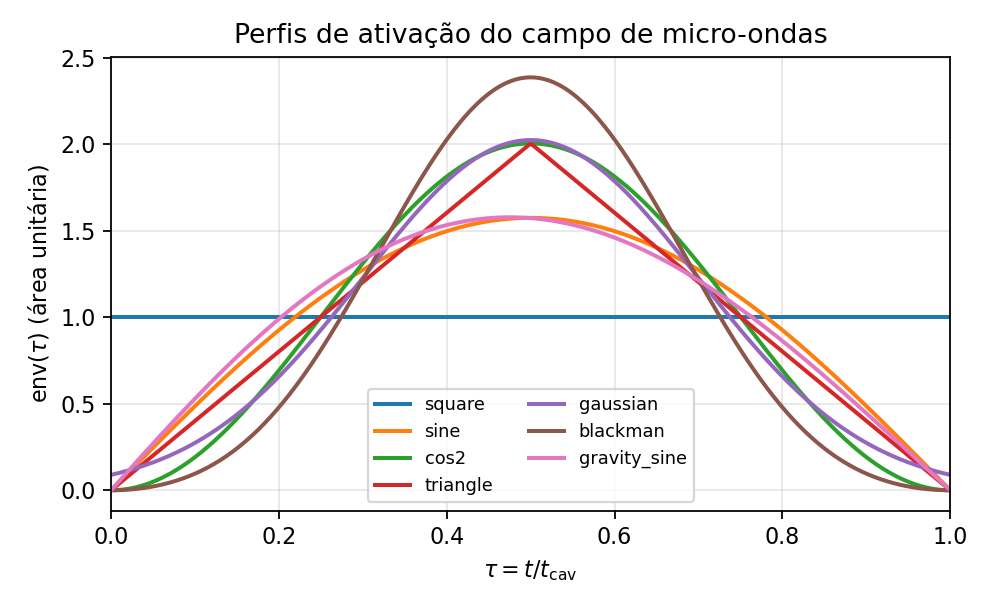
\includegraphics[width=0.62\textwidth]{figuras/fig_perfis.png}
  \caption{Os sete perfis de ativação do campo de micro-ondas, normalizados para área
  unitária.}
  \label{fig:perfis}
\end{figure}

\begin{figure}[htbp]
  \centering
  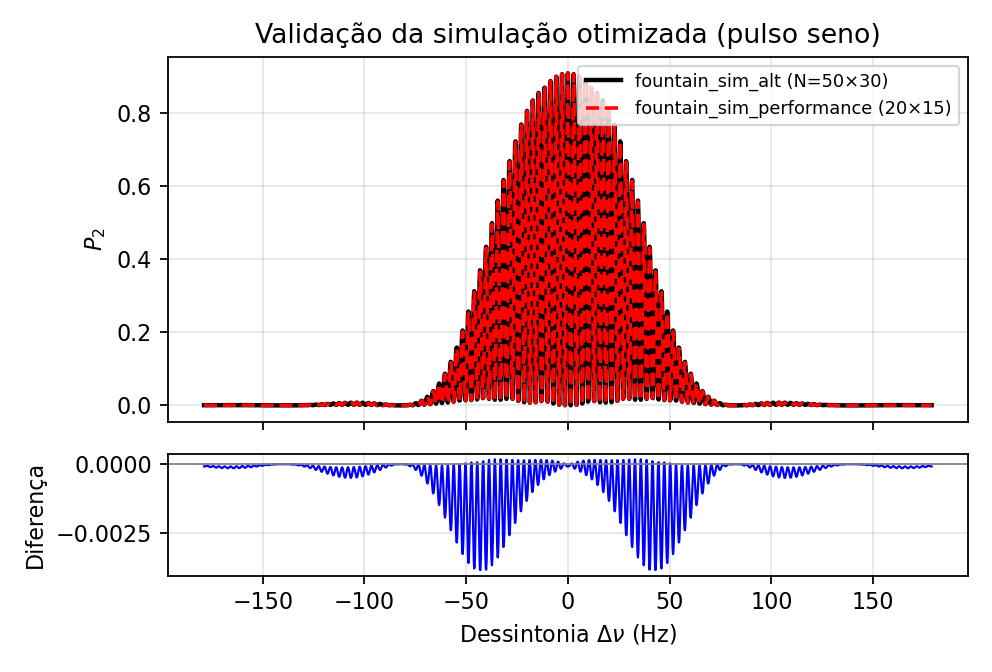
\includegraphics[width=0.62\textwidth]{figuras/fig_validacao.png}
  \caption{Validação da simulação otimizada (linha tracejada) contra
  \texttt{fountain\_sim\_alt} (linha contínua) para o pulso seno. O painel inferior mostra a
  diferença, da ordem de $10^{-3}$.}
  \label{fig:validacao}
\end{figure}

\begin{figure}[htbp]
  \centering
  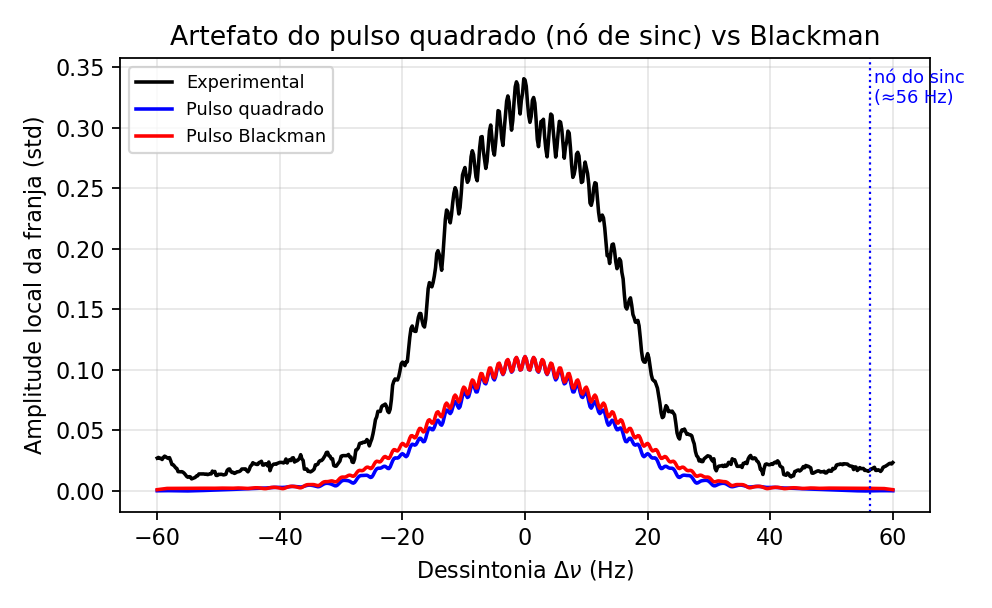
\includegraphics[width=0.62\textwidth]{figuras/fig_no_sinc.png}
  \caption{Amplitude local da franja em função da dessintonia. O pulso quadrado (azul)
  colapsa a franja no nó de sinc em $\approx 56$\,Hz, enquanto o Blackman (vermelho) decai
  suavemente, acompanhando o dado experimental (preto).}
  \label{fig:nosinc}
\end{figure}

\section{Código de ajuste (\texttt{fit\_data.py})}
O código de ajuste foi reescrito em torno da modelagem da \textbf{resposta instrumental
linear} do detector.

\subsection{Resposta instrumental linear}
O sinal bruto medido não é a probabilidade $P_2$ diretamente, mas sim
\begin{equation}
  y_{\mathrm{obs}} = A\,P_2(\Delta\nu;\ \text{físicos}) + C,
  \label{eq:resposta}
\end{equation}
onde $A$ é o \emph{contraste/escala} (eficiência de detecção, ganho) e $C$ é o
\emph{fundo/offset} (átomos não-bombeados, luz espalhada, corrente escura). Como $A$ e $C$
são \textbf{lineares}, eles são \emph{perfilados} analiticamente a cada iteração por
mínimos quadrados:
\begin{equation}
  A = \frac{\sum_i (P_{2,i}-\bar P_2)(y_i-\bar y)}{\sum_i (P_{2,i}-\bar P_2)^2},
  \qquad
  C = \bar y - A\,\bar P_2 .
\end{equation}
Assim, o otimizador não-linear permanece apenas com os parâmetros físicos
$\{\mathrm{Temp},\,T,\,\tau\}$ (com $\theta=\pi/2$ fixo), e o resíduo é
\begin{equation}
  r_i = \big(A\,P_{2,i} + C\big) - y_i .
\end{equation}

Esse procedimento elimina a distorção da normalização min--max anterior, que forçava o
mínimo e o máximo ruidosos do sinal a $0$ e $1$, respectivamente.

\subsection{Estratégia de ajuste e seleção de modelo}
O ajuste usa \texttt{scipy.optimize.least\_squares} em duas fases (multistart grosseiro com
resolução reduzida, seguido de refinamento), e o tempo de voo livre $T$ é estimado
inicialmente pela frequência dominante das franjas via FFT. Para cada um dos sete perfis,
o ajuste é repetido e as métricas são comparadas (seleção de modelo).

\section{Métricas de eficácia}
Três métricas quantificam a qualidade do ajuste. Definindo o resíduo $r_i = y_{\mathrm{fit},i}
- y_i$, a soma dos quadrados dos resíduos $SS_{\mathrm{res}} = \sum_i r_i^2$ e a soma dos
quadrados totais $SS_{\mathrm{tot}} = \sum_i (y_i - \bar y)^2$:

\begin{itemize}
  \item \textbf{Coeficiente de determinação} $R^2 = 1 - SS_{\mathrm{res}}/SS_{\mathrm{tot}}$:
        fração da variância explicada pelo modelo (próximo de $1$ é melhor);
  \item \textbf{Raiz do erro quadrático médio} $\mathrm{RMSE} = \sqrt{\frac{1}{n}\sum_i r_i^2}$:
        erro típico em unidades do sinal (menor é melhor);
  \item \textbf{Critério de informação de Akaike}
        $\mathrm{AIC} = n\ln(SS_{\mathrm{res}}/n) + 2k$, com $k$ o número de parâmetros:
        penaliza complexidade e permite comparar modelos (menor é melhor).
\end{itemize}

Além das métricas globais, analisa-se o \textbf{resíduo na região de \emph{washing-out}}
($15$--$45$\,Hz), onde os padrões de interferência destrutiva (vales) são mais sensíveis ao
desalinhamento vertical entre modelo e dados.

\section{Resultados}

\subsection{Melhoria pela resposta instrumental}
A Figura~\ref{fig:antesdepois} compara a abordagem anterior (normalização min--max) com a
resposta instrumental linear. O $R^2$ global sobe de $0{,}797$ para $0{,}981$, e o RMSE na
região de washing-out cai substancialmente. O offset $C \approx -0{,}427$ coincide com a
linha de base do sinal bruto ($\approx -0{,}43$), assentando corretamente os \textbf{vales de
interferência destrutiva}.

\begin{figure}[htbp]
  \centering
  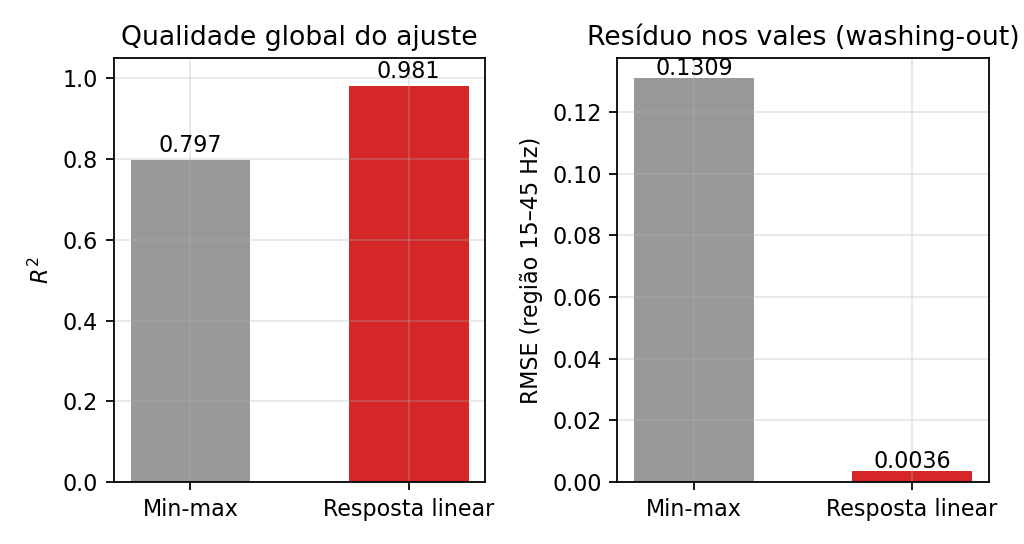
\includegraphics[width=0.72\textwidth]{figuras/fig_antes_depois.png}
  \caption{Comparação entre a normalização min--max (cinza) e a resposta instrumental linear
  (vermelho). Esquerda: $R^2$ global. Direita: RMSE na região de washing-out ($15$--$45$\,Hz).}
  \label{fig:antesdepois}
\end{figure}

\subsection{Ajuste final}
A Figura~\ref{fig:ajuste} mostra o ajuste final (melhor perfil, \texttt{square}) sobre o sinal
bruto, com o subplot de resíduos. O resíduo é aproximadamente homogêneo e da ordem de
$10^{-3}$, indicando que o modelo captura tanto os picos quanto os vales do padrão de
interferência.

\begin{figure}[htbp]
  \centering
  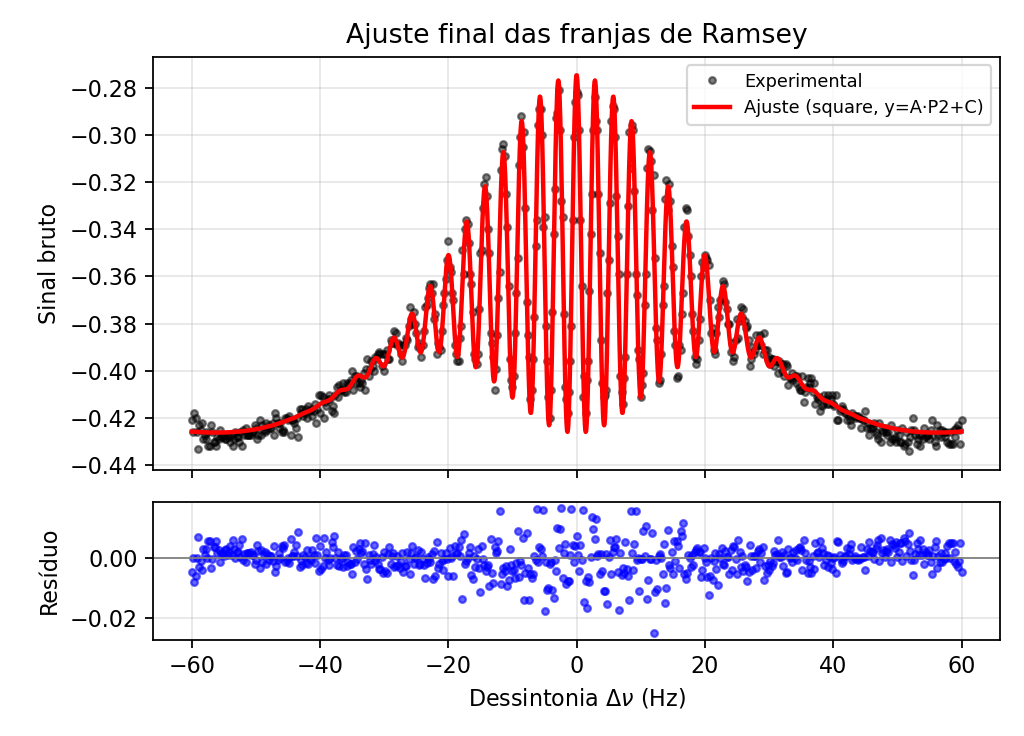
\includegraphics[width=0.72\textwidth]{figuras/fig_ajuste_final.png}
  \caption{Ajuste final (perfil \texttt{square}, $y = A\,P_2 + C$). Painel superior: sinal
  experimental (pontos) e modelo ajustado (linha). Painel inferior: resíduo.}
  \label{fig:ajuste}
\end{figure}

\subsection{Seleção de modelo}
A Tabela~\ref{tab:selecao} e a Figura~\ref{fig:selecao} resumem a seleção de modelo entre os
sete perfis. Todos apresentam $R^2 \approx 0{,}978$--$0{,}981$, indicando que os dados
\textbf{não discriminam fortemente} o perfil de ativação (como esperado: o envelope das
franjas depende de vários efeitos simultâneos). O perfil \texttt{square} vence por margem
mínima, embora os perfis suaves (sine, gravity\_sine) sejam fisicamente mais plausíveis.

\begin{table}[htbp]
  \centering
  \begin{tabular}{lccccc}
    \toprule
    Perfil & $R^2$ & RMSE & AIC & Temp.\ ($\mu$K) & $\tau$ (s) \\
    \midrule
    square       & 0{,}981254 & 0{,}005021 & $-6353{,}6$ & 64{,}3 & 0{,}01758 \\
    sine         & 0{,}979970 & 0{,}005190 & $-6313{,}8$ & 72{,}6 & 0{,}02361 \\
    gravity\_sine& 0{,}979957 & 0{,}005192 & $-6313{,}4$ & 72{,}7 & 0{,}02362 \\
    cos2         & 0{,}979117 & 0{,}005299 & $-6288{,}7$ & 80{,}9 & 0{,}02874 \\
    triangle     & 0{,}978991 & 0{,}005315 & $-6285{,}1$ & 76{,}0 & 0{,}02533 \\
    blackman     & 0{,}978089 & 0{,}005428 & $-6259{,}8$ & 88{,}5 & 0{,}03274 \\
    gaussian     & 0{,}978003 & 0{,}005439 & $-6257{,}5$ & 80{,}1 & 0{,}02741 \\
    \bottomrule
  \end{tabular}
  \caption{Resultados da seleção de modelo (resposta instrumental linear, $\theta=\pi/2$
  fixo). $A\approx 0{,}50$--$0{,}52$ e $C\approx -0{,}427$ para todos os perfis.}
  \label{tab:selecao}
\end{table}

\begin{figure}[htbp]
  \centering
  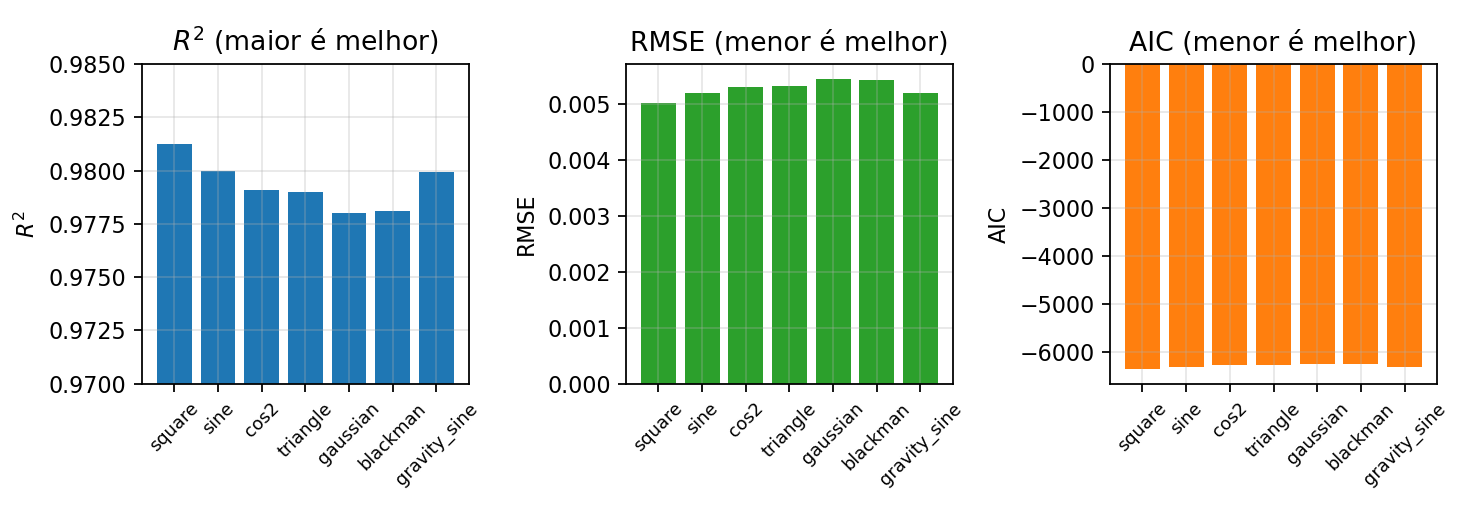
\includegraphics[width=0.95\textwidth]{figuras/fig_selecao_modelo.png}
  \caption{Seleção de modelo: $R^2$ (maior é melhor), RMSE e AIC (menores são melhores) para
  os sete perfis de ativação.}
  \label{fig:selecao}
\end{figure}

\subsection{Diagnóstico físico da temperatura}
Com a amplitude desacoplada pela resposta instrumental (parâmetro $A$), a temperatura
convergiu para $\approx 64$--$88\,\mu$K, bem acima do valor físico esperado de
$\approx 1\,\mu$K. Isso é um \textbf{diagnóstico importante}: o mecanismo de
\emph{washing-out} do modelo (defasagem por dispersão de velocidades) é fraco demais a
$1\,\mu$K, e o ajuste compensa inflando a temperatura. Indica um mecanismo de lavagem
\emph{não modelado} (ex.: gradiente de campo $B$, tamanho finito da nuvem ou temperatura
anisotrópica).

\section{Conclusão}
Foi desenvolvida e validada uma metodologia completa de ajuste das franjas de Ramsey de um
chafariz atômico. Os três avanços centrais são:

\begin{enumerate}
  \item uma simulação \textbf{otimizada} ($9$--$14\times$ mais rápida, erro $<0{,}4\%$) com
        sete perfis de ativação fisicamente motivados;
  \item a modelagem da \textbf{resposta instrumental linear} $y = A\,P_2 + C$, que elevou o
        $R^2$ de $0{,}80$ para $0{,}98$ e assentou os vales de interferência destrutiva;
  \item um procedimento de \textbf{seleção de modelo} com métricas objetivas ($R^2$, RMSE,
        AIC).
\end{enumerate}

As métricas comprovam a viabilidade do método, e o diagnóstico da temperatura aponta para
futuras extensões físicas do modelo (gradiente de campo magnético, nuvem finita).

\end{document}


